%!TEX root = ../Thesis.tex

\section{Problem 3}
\label{sec:problem_3}%

In this final problem we search for the solution of a simple potential problem with mixed boundary conditions. The interesting thing is that the square domain $\Omega$ is doubly connected, namely, it contains a hole. Its outer boundary has been discretized into 16 constant elements, while the inner one into 8 elements. The solution is sought at 8 internal points. The data and the boundary discretization are shown in Fig.~\ref{fig:2pr3f1} and Fig.~\ref{fig:2pr3f2}.

\begin{figure}[H]
    \centering
    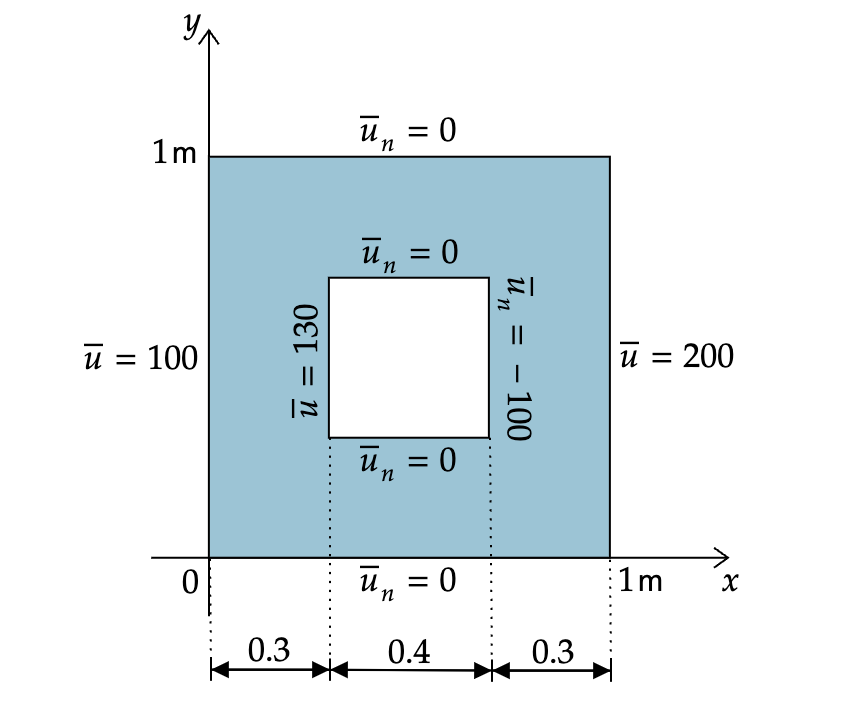
\includegraphics[width=0.6\textwidth]{pr3f1}
    \caption{Doubly connected square domain $\Omega$ and boundary conditions of Problem 3.}
    \label{fig:2pr3f1}
\end{figure}

\begin{figure}[H]
    \centering
    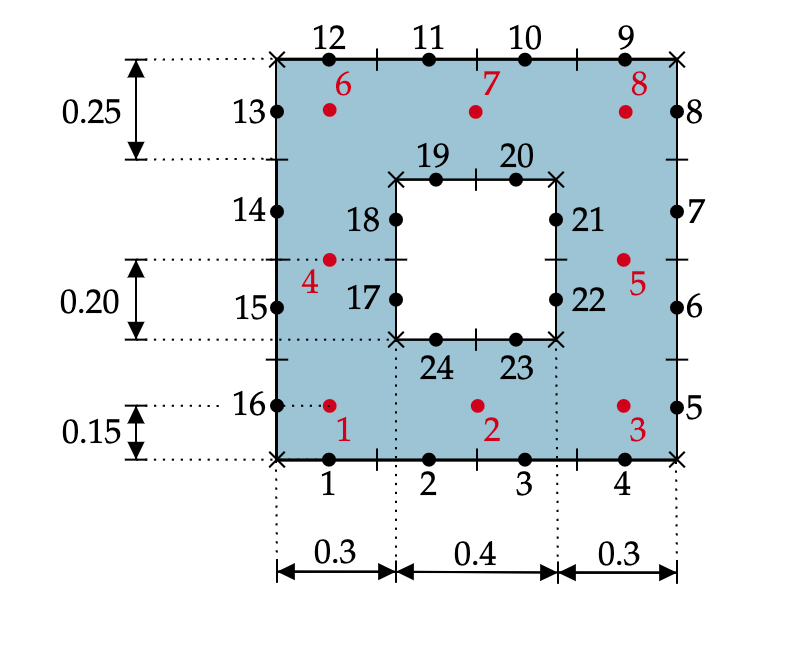
\includegraphics[width=0.6\textwidth]{pr3f2}
    \caption{Boundary element discretization and internal points (in red) of Problem 3.}
    \label{fig:2pr3f2}
\end{figure}

\subsection{MATLAB Implementation}
\label{sub:MATLAB_implementation4}%

The program we used to solve Problem 1 and 2 can be readily modified to solve potential problems in multiply connected domains (domains with holes). The changes affect only the functions \texttt{MIDPOINTS} (see Algorithm~\ref{alg:holeMIDPOINTS}), \texttt{GMATR} (see Algorithm~\ref{alg:holeGMATR}), \texttt{HMATR} (see Algorithm~\ref{alg:holeHMATR}), \texttt{UINTER} (see Algorithm~\ref{alg:holeUINTER}) and of course the print functions, while the overall structure of the \texttt{main} script (see Algorithm~\ref{alg:main23}) remains as before (see Eq.~\eqref{eq:flowchart}). We only added two new parameters to the ones already presented in Table~\ref{table:2pr1t1}. One is NB and it defines the number of boundaries, the second is the vector NL($i$) which identifies the number of the last element on the $i$-th boundary ($i=1,\dots,\text{NB}$). It should also be noted that the elements of all the boundaries are numbered consecutively and, therefore, N denotes the total number of elements.

The output of the program is the following:
\begin{matlaboutput}
*********************************************************************
RESULTS
*********************************************************************

BOUNDARY NODES:

NODE        XM            YM            U                   U_n
 1        0.12500       0.00000    1.121172e+02           0.00000
 2        0.37500       0.00000    1.377572e+02           0.00000
 3        0.62500       0.00000    1.627310e+02           0.00000
 4        0.87500       0.00000    1.881075e+02           0.00000
 5        1.00000       0.12500             200         105.36171
 6        1.00000       0.37500             200          95.21982
 7        1.00000       0.62500             200          95.21982
 8        1.00000       0.87500             200         105.36171
 9        0.87500       1.00000    1.881075e+02           0.00000
 10       0.62500       1.00000    1.627310e+02           0.00000
 11       0.37500       1.00000    1.377572e+02           0.00000
 12       0.12500       1.00000    1.121172e+02           0.00000
 13       0.00000       0.87500             100        -107.76583
 14       0.00000       0.62500             100         -99.55986
 15       0.00000       0.37500             100         -99.55986
 16       0.00000       0.12500             100        -107.76583
---------------------------------------------------------------------
 17       0.30000       0.40000             130         108.32831
 18       0.30000       0.60000             130         108.32831
 19       0.40000       0.70000    1.405389e+02           0.00000
 20       0.60000       0.70000    1.600210e+02           0.00000
 21       0.70000       0.60000    1.716784e+02        -100.00000
 22       0.70000       0.40000    1.716784e+02        -100.00000
 23       0.60000       0.30000    1.600210e+02           0.00000
 24       0.40000       0.30000    1.405389e+02           0.00000

INTERNAL POINTS:

POINT        XIN           YIN           U
  1        0.15000       0.15000     115.08022
  2        0.50000       0.15000     150.26437
  3        0.85000       0.15000     185.25460
  4        0.15000       0.50000     115.07475
  5        0.85000       0.50000     185.68733
  6        0.15000       0.85000     115.08022
  7        0.50000       0.85000     150.26437
  8        0.85000       0.85000     185.25460
\end{matlaboutput} 

\subsection{MATLAB scripts}
\label{sub:matlab_scripts4}%

\begin{matlab}{holeMIDPOINTS}{alg:holeMIDPOINTS}
function [XM, YM] = holeMIDPOINTS(XL, YL, NB, NL)
XM = zeros(NL(end),1);
YM = zeros(NL(end),1);
beg = 1;
for i = 1:NB
    for j = beg:NL(i)
        if j==NL(i)
            XM(j) = (XL(j)+XL(beg))/2;
            YM(j) = (YL(j)+YL(beg))/2;
        else
            XM(j) = (XL(j)+XL(j+1))/2;
            YM(j) = (YL(j)+YL(j+1))/2;
        end
    end
    beg = NL(i)+1;
end
end
\end{matlab}

\begin{matlab}{holeGMATR}{alg:holeGMATR}
function G = holeGMATR(XL, YL, XM, YM, N, NB, NL)
G = zeros(N,N); beg = 1;
for k = 1:NB
    for i = 1:N
        for j = beg:NL(k)
            if i~=j % off-diagonal elements of G
                if j==NL(k)
                    G(i,j) = RLINTC(XM(i),YM(i),XL(j),YL(j),XL(beg),YL(beg));


                else
                    G(i,j) = RLINTC(XM(i),YM(i),XL(j),YL(j),XL(j+1),YL(j+1));
                end
            elseif i==j % diagonal elements of G
                if j==NL(k)
                    G(i,j) = SLINTC(XL(j),YL(j),XL(beg),YL(beg));
                else
                    G(i,j) = SLINTC(XL(j),YL(j),XL(j+1),YL(j+1));
                end
            end
        end
    end
    beg = NL(k)+1;
end
end
\end{matlab}

\begin{matlab}{holeHMATR}{alg:holeHMATR}
function H = holeHMATR(XL, YL, XM, YM, N, NB, NL)
H = zeros(N,N);
beg = 1;
for k=1:NB
    for i = 1:N
        for j = beg:NL(k)
            if i~=j % off-diagonal elements of G
                if j==NL(k)
                    H(i,j) = DALPHA(XM(i),YM(i),XL(j),YL(j),XL(beg),YL(beg));
                else
                    H(i,j) = DALPHA(XM(i),YM(i),XL(j),YL(j),XL(j+1),YL(j+1));
                end
            elseif i == j % diagonal elements of G
                H(i,j) = -0.5;
            end
        end
    end
    beg = NL(k)+1;
end
end
\end{matlab}

\newpage

\begin{matlab}{holeUINTER}{alg:holeUINTER}
function UIN = holeUINTER(XL, YL, XIN, YIN, UB, UNB, N, IN, NL, NB)
UIN = zeros(IN, 1);
for k = 1:IN
    for j = 1:N
        if NB == 1
            resh = DALPHA(XIN(k), YIN(k), XL(j), YL(j), XL(j+1), YL(j+1));
            resg = RLINTC(XIN(k), YIN(k), XL(j), YL(j), XL(j+1), YL(j+1));
            UIN(k) = UIN(k) + resh*UB(j) - resg*UNB(j);
        else
            if j == NL(1)
                resh = DALPHA(XIN(k), YIN(k), XL(j), YL(j), XL(1), YL(1));
                resg = RLINTC(XIN(k), YIN(k), XL(j), YL(j), XL(1), YL(1));
                UIN(k) = UIN(k) + resh*UB(j) - resg*UNB(j);
            else
                for kk = 2:NB
                    if j == NL(kk)
                        resh = DALPHA(XIN(k), YIN(k), XL(j), YL(j), XL( NL(kk-1)+1  ), YL( NL(kk-1)+1 ));
                        resg = RLINTC(XIN(k), YIN(k), XL(j), YL(j),  XL( NL(kk-1)+1  ), YL( NL(kk-1)+1 ));
                        UIN(k) = UIN(k) + resh*UB(j) - resg*UNB(j);
                    else
                        resh = DALPHA(XIN(k), YIN(k), XL(j), YL(j), XL(j+1), YL(j+1));
                        resg = RLINTC(XIN(k), YIN(k), XL(j), YL(j), XL(j+1), YL(j+1));
                        UIN(k) = UIN(k) + resh*UB(j) - resg*UNB(j);
                    end
                end
            end
        end

    end
end
end
\end{matlab}

\begin{matlab}{main23}{alg:main23}
%% Problem 2 - Square hole in a square
clear; clc; 


% Set the maximum dimensions
N = 24;
IN = 8;
NB = 2; % # boundaries
NL = [16; 24]; % last point of each boundary

% Set data
XL = [0; 0.25; 0.5; 0.75; 1; 1; 1; 1; 1; 0.75; 0.5; 0.25; 0; 0; 0; 0;
      0.3; 0.3; 0.3; 0.5; 0.7; 0.7; 0.7; 0.5];
YL = [0; 0; 0; 0; 0; 0.25; 0.5; 0.75; 1; 1; 1; 1; 1; 0.75; 0.5; 0.25;
      0.3; 0.5; 0.7; 0.7; 0.7; 0.5; 0.3; 0.3];
INDEX = [1; 1; 1; 1; 0; 0; 0; 0; 1; 1; 1; 1; 0; 0; 0; 0; 
         0; 0; 1; 1; 1; 1; 1; 1];
UB = [0; 0; 0; 0; 200; 200; 200; 200; 0; 0; 0; 0; 100; 100; 100; 100; 
      130; 130; 0; 0; -100; -100; 0; 0];
XIN = [0.15; 0.5; 0.85; 0.15; 0.85; 0.15; 0.5; 0.85];
YIN = [0.15; 0.15; 0.15; 0.5; 0.5; 0.85; 0.85; 0.85];

% Compute midpoints
[XM, YM] = holeMIDPOINTS(XL, YL, NB, NL);

% Print data
holeINPUT(XL, YL, XM, YM, XIN, YIN, INDEX, UB, N, IN, NB, NL);

% % Compute the G matrix
G = holeGMATR(XL, YL, XM, YM, N, NB, NL);

% Compute the H matrix
H = holeHMATR(XL, YL, XM, YM, N, NB, NL);

% Form the system of equations AX=B
[A, UNB] = ABMATR(G, H, UB, INDEX);

% Solve the system of equations
UNB = A\UNB;

% Form the vectors U and UN of all the boundary values
[UB, UNB] = REORDER(UB, UNB, INDEX);

% Compute the values UIN of u at the internal points
UIN = holeUINTER(XL, YL, XIN, YIN, UB, UNB, N, IN, NL, NB);

% Print results
holeOUTPUT(XM, YM, XIN, YIN, UB, UNB, UIN, N, IN, NL, NB);
\end{matlab}

\subsection{Abaqus Implementation}
\label{sub:Abaqus_implementation4}%

The Abaqus procedure is symmetric to the ones of Problem 2, and described in Section~\ref{sub:Abaqus_implementation3}. Let us mention the main passages:
\begin{itemize}
\item Part module: we create a 2D planar deformable shell part of size 2000, then we create the square with a hole.
%foto 1
\begin{figure}[H]
    \centering
    
\includegraphics[width=0.5\textwidth]{Images/ab3/ab1.png}
    \caption{Final result of Part module.}
    \label{fig:abb1}
\end{figure}

\item Property module: we define a material with conductivity $k=1000$ (see Eq.~\eqref{eq:conductivity}) and we assign it to a solid homogeneous section.

\item Assemply module: we create a dependent instance.

\item Step module: we define a steady state heat transfer step.

\item Load module: we assign the boundary conditions.
% foto 2 + 3
\begin{figure}[H]
    \centering
    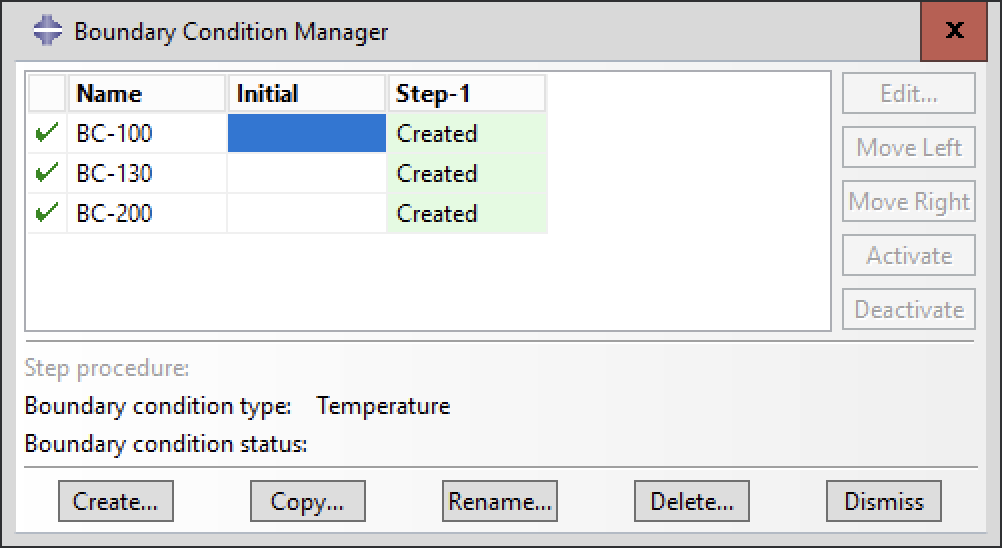
\includegraphics[width=0.55\textwidth]{Images/ab3/ab2.png} \qquad 
    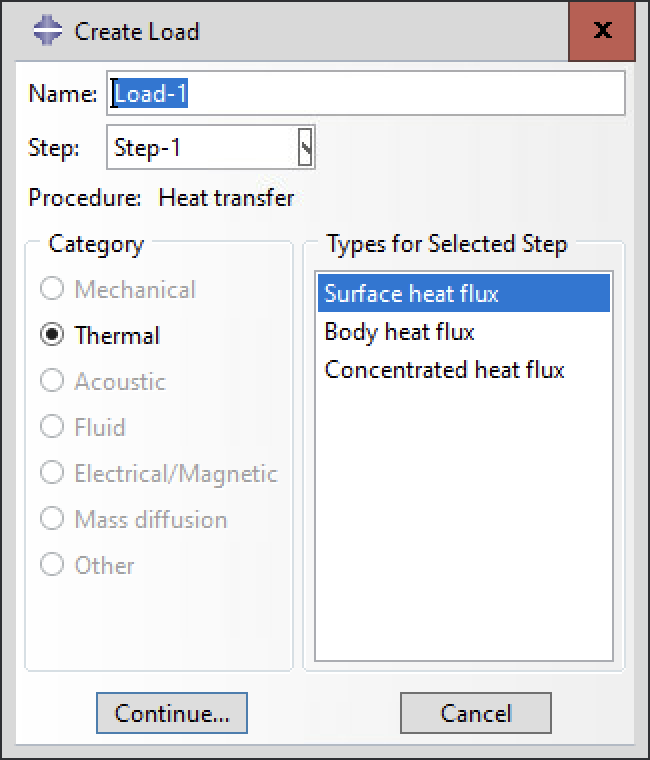
\includegraphics[width=0.26\textwidth]{Images/ab3/ab3.png}
    \caption{Boundary conditions.}
    \label{fig:abb23}
\end{figure}

This is what we obtained so far:
% foto 4
\begin{figure}[H]
    \centering
    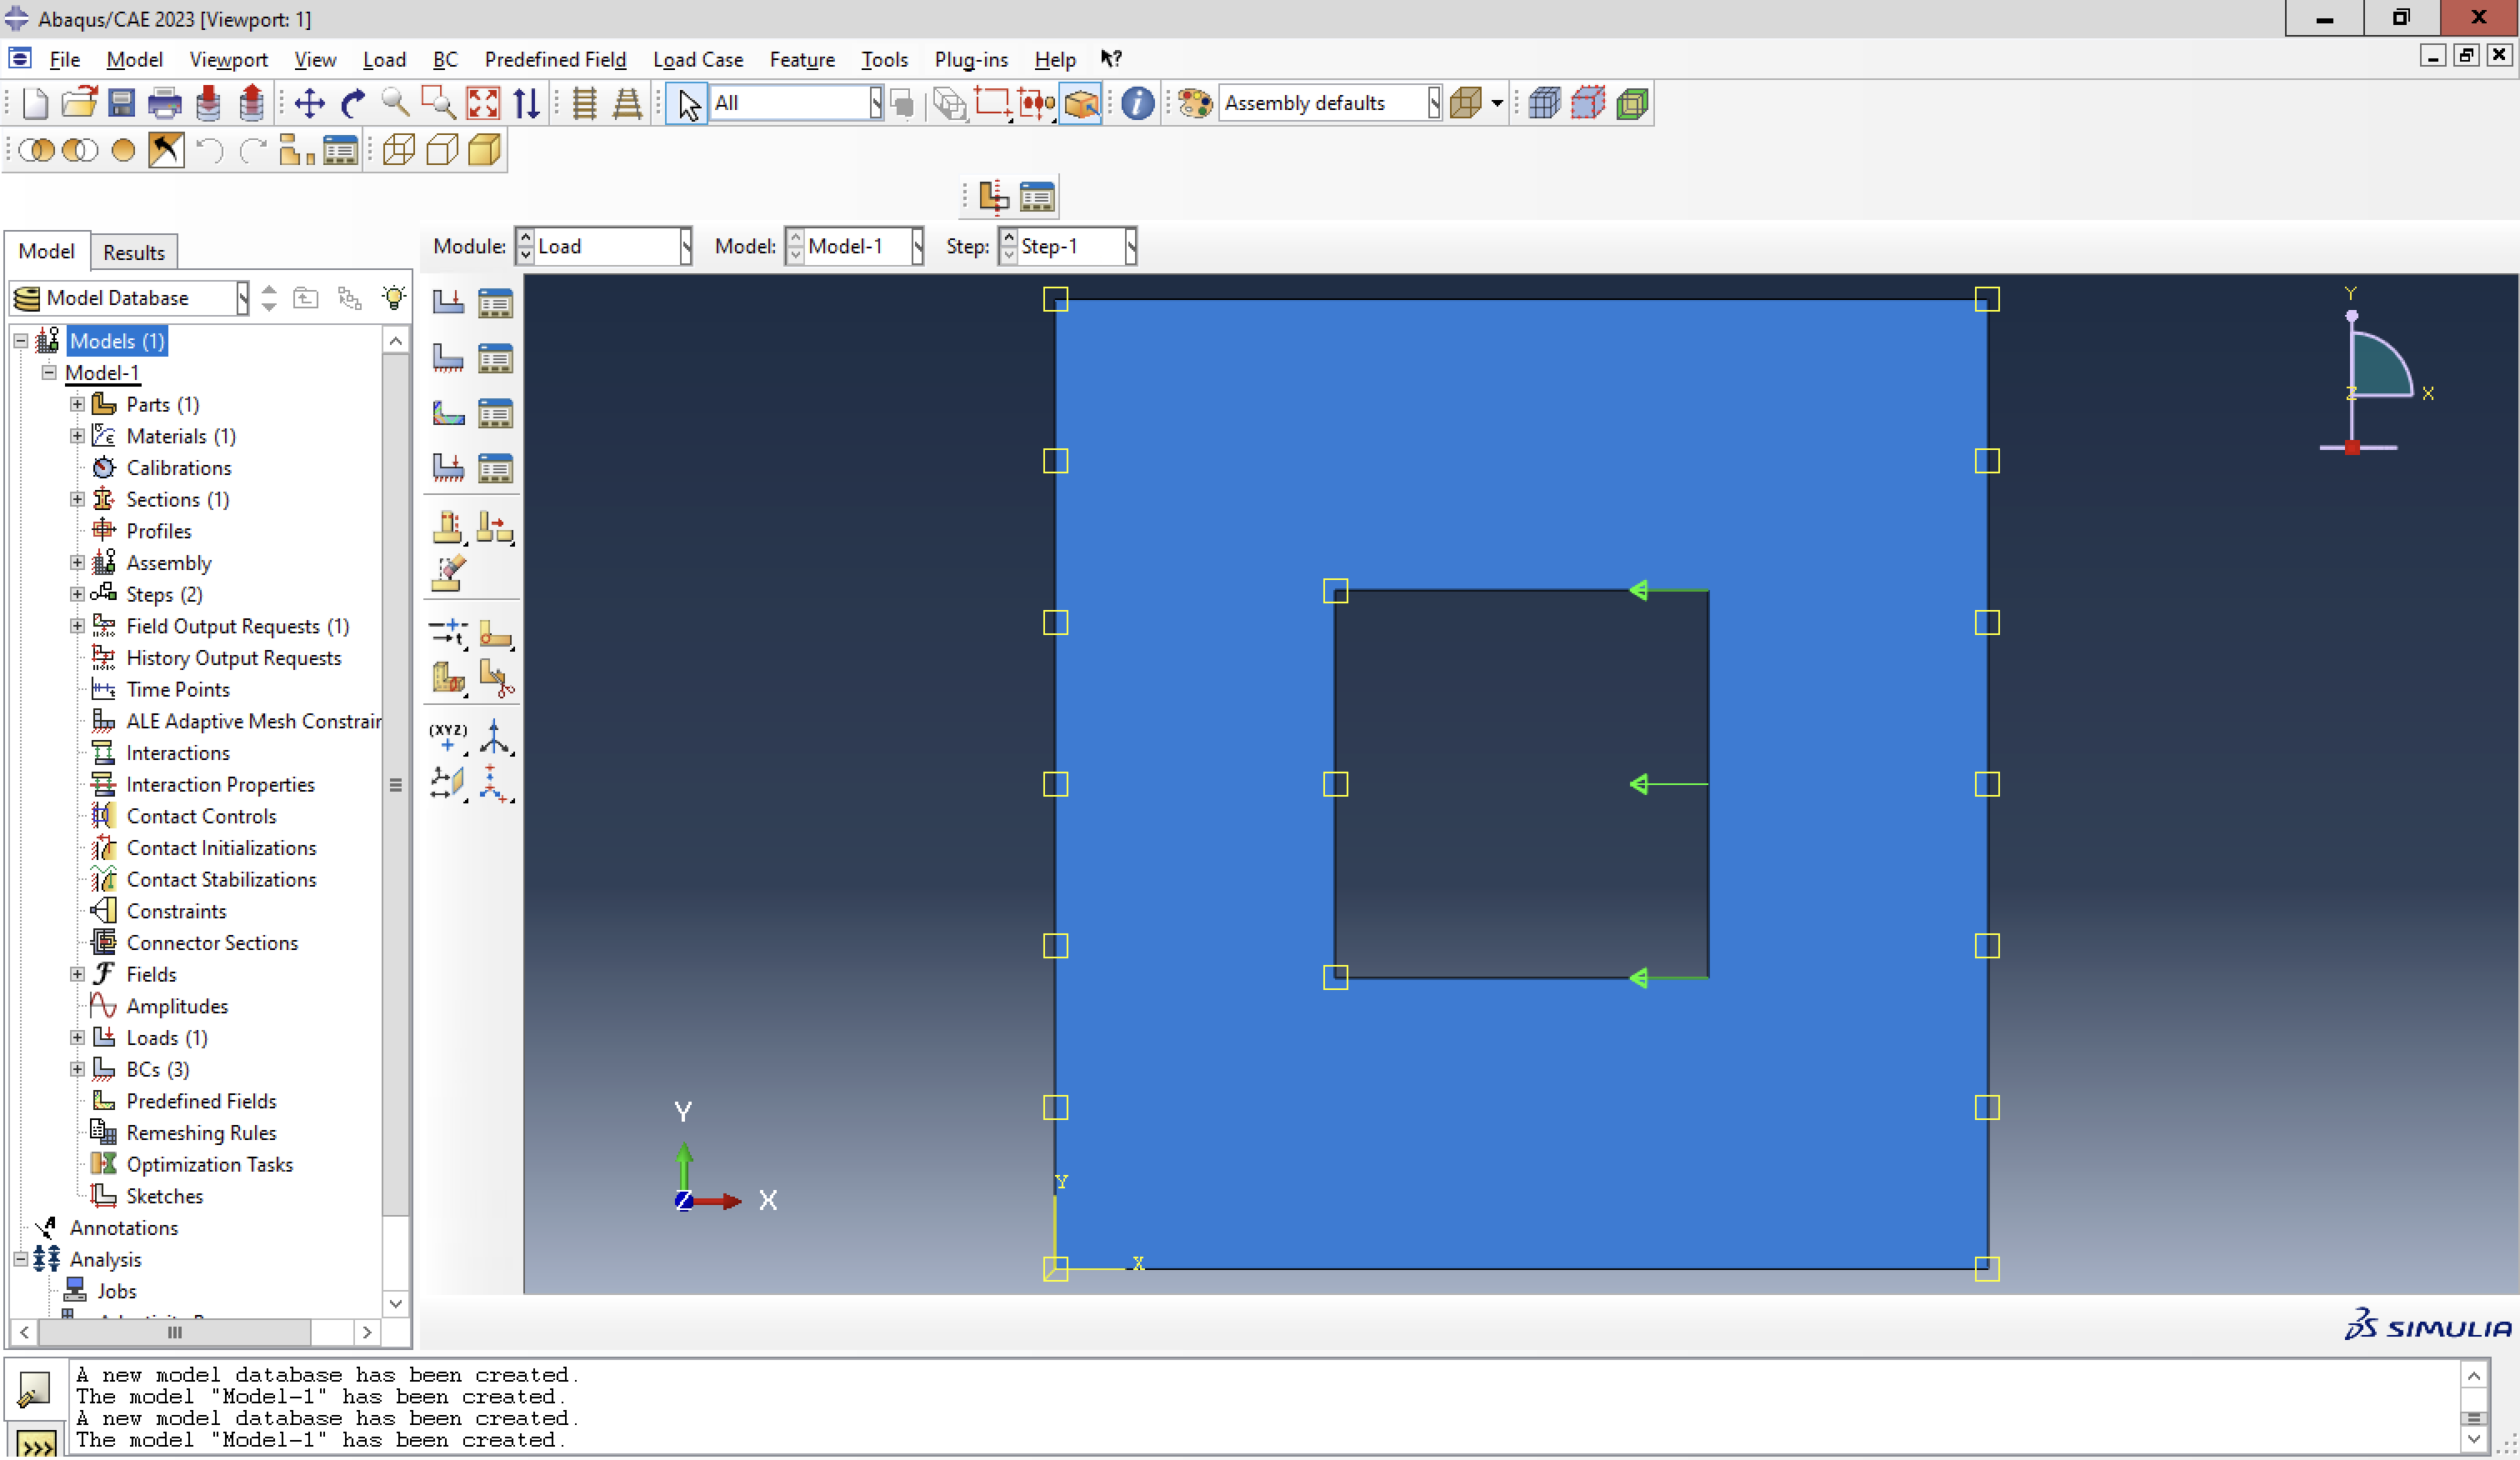
\includegraphics[width=\textwidth]{Images/ab3/ab4.png}
    \caption{Final result of Load module.}
    \label{fig:abb4}
\end{figure}

\item Mesh module: we assign the heat transfer element type, then in Mesh Controls we set the quad shape and the medial axis algorithm.
% foto 5
\begin{figure}[H]
    \centering
    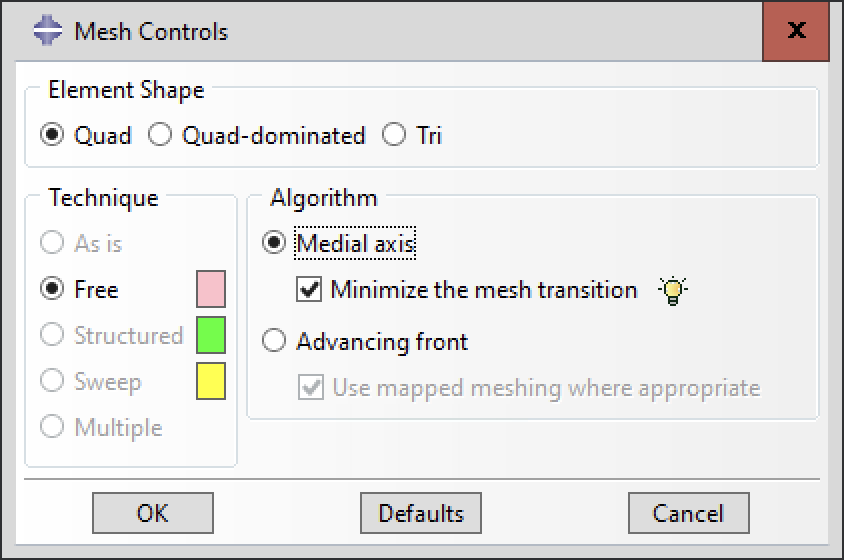
\includegraphics[width=0.6\textwidth]{Images/ab3/ab5.png}
    \caption{Mesh Controls.}
    \label{fig:abb5}
\end{figure}

\newpage

In the Global Seeds option, we define a length of 50 mm for the quads edges: $1000\,\text{mm}/50\,\text{mm}=20$ global size.
% foto 6
\begin{figure}[H]
    \centering
    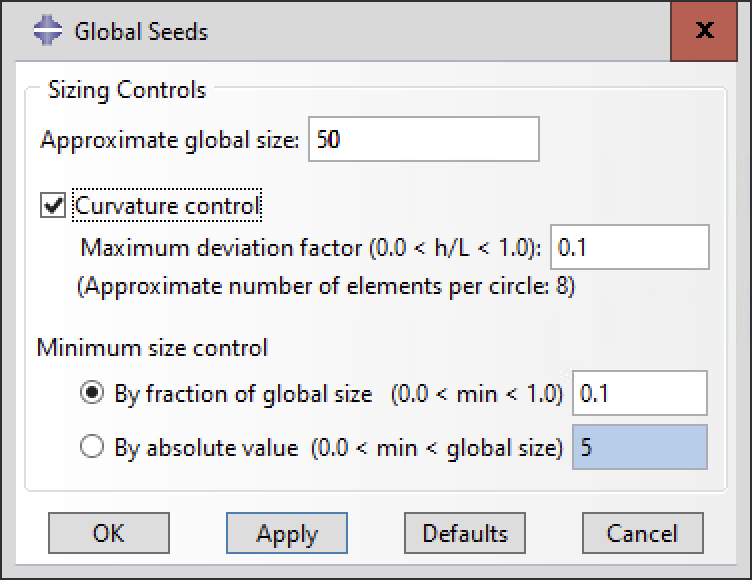
\includegraphics[width=0.5\textwidth]{Images/ab3/ab6.png}
    \caption{Global Seeds.}
    \label{fig:abb6}
\end{figure}

Here the final mesh:
% foto 7
\begin{figure}[H]
    \centering
    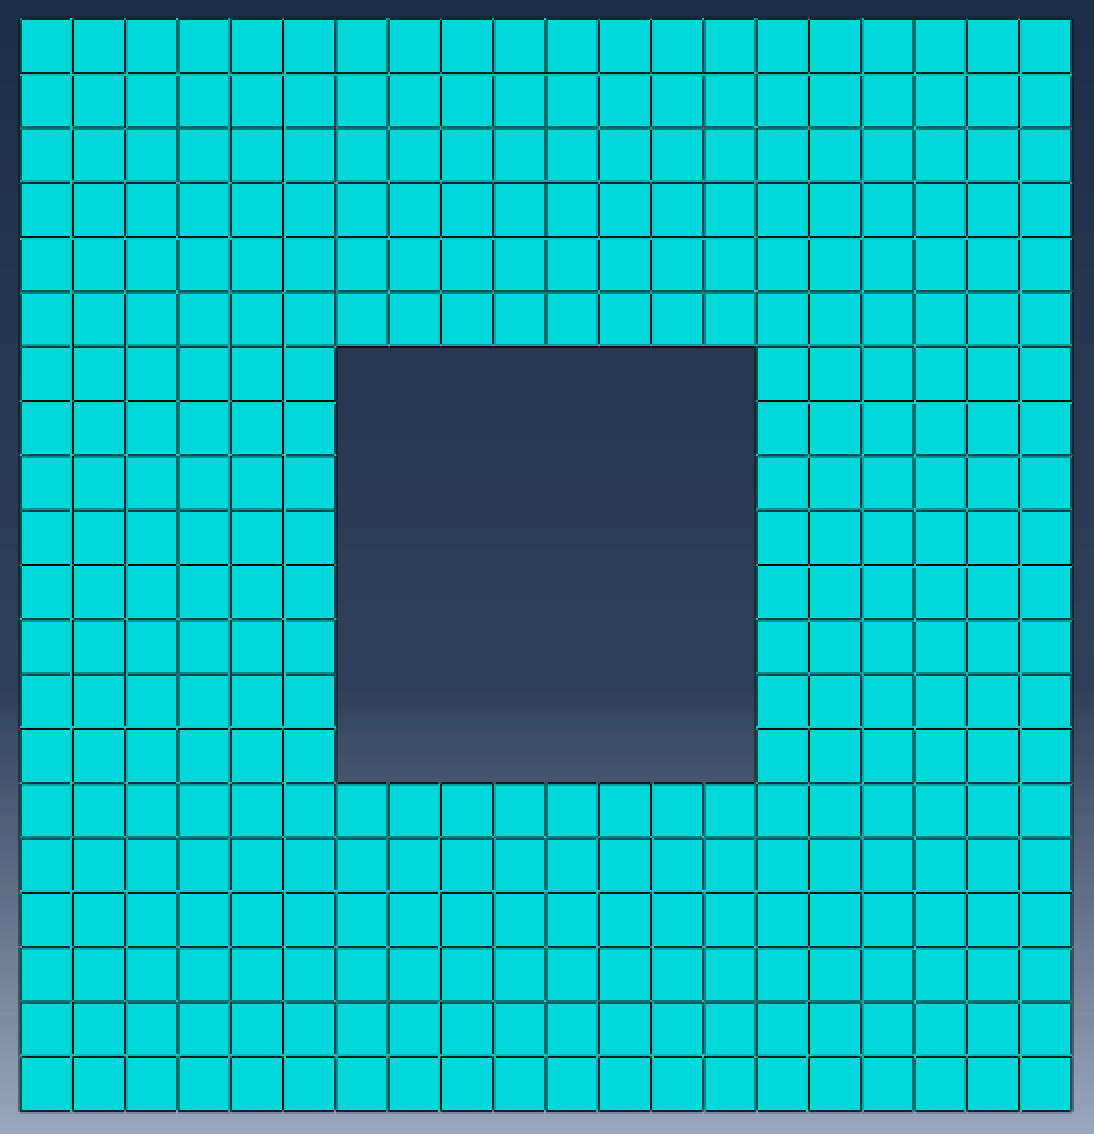
\includegraphics[width=0.65\textwidth]{Images/ab3/ab7.png}
    \caption{Final result of Mesh module.}
    \label{fig:abb7}
\end{figure}

\item Job module: finaly, we submit a standard job.
\end{itemize}

In the Visualization module, we observe the nodal temperature distributions:
% foto 8
\begin{figure}[H]
    \centering
    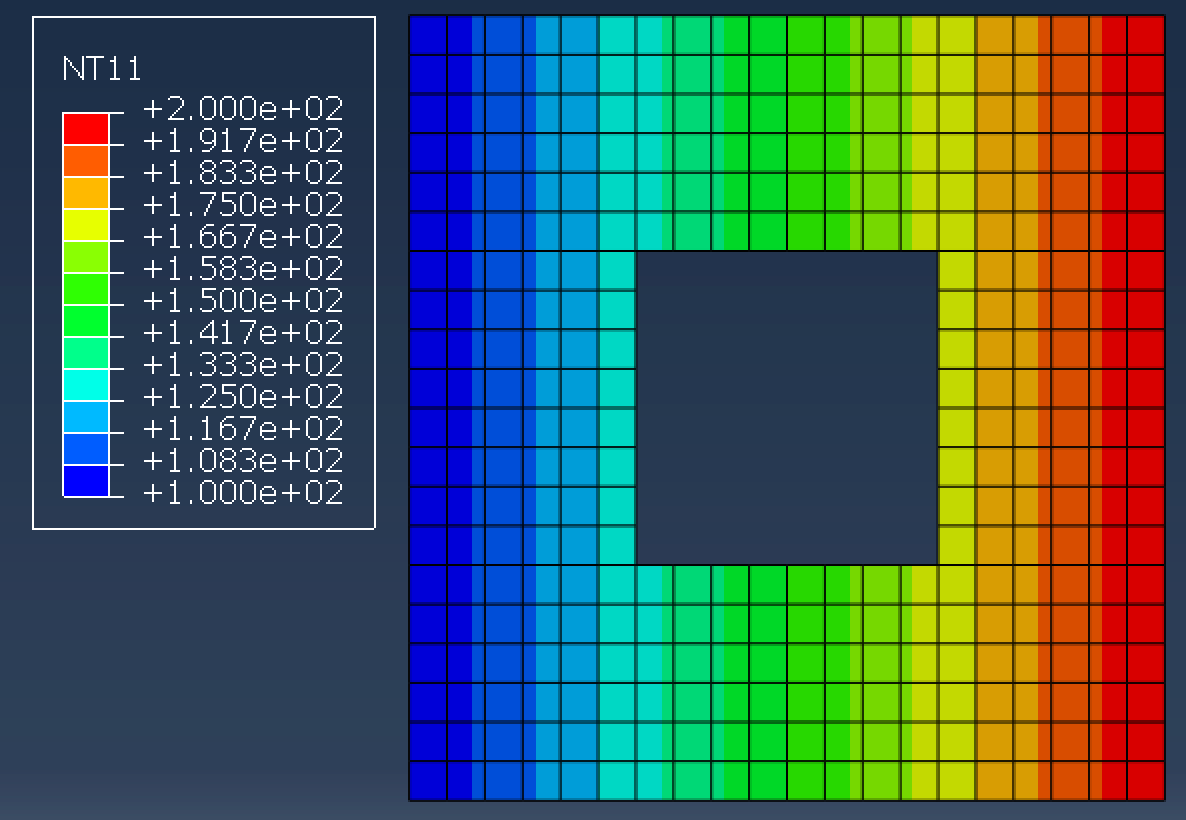
\includegraphics[width=0.8\textwidth]{Images/ab3/ab8.png}
    \caption{Nodal temperature.}
    \label{fig:abb8}
\end{figure}

Then, we extract the numerical values of the eight internal points:
% foto 10 + 11
\begin{figure}[H]
    \centering
    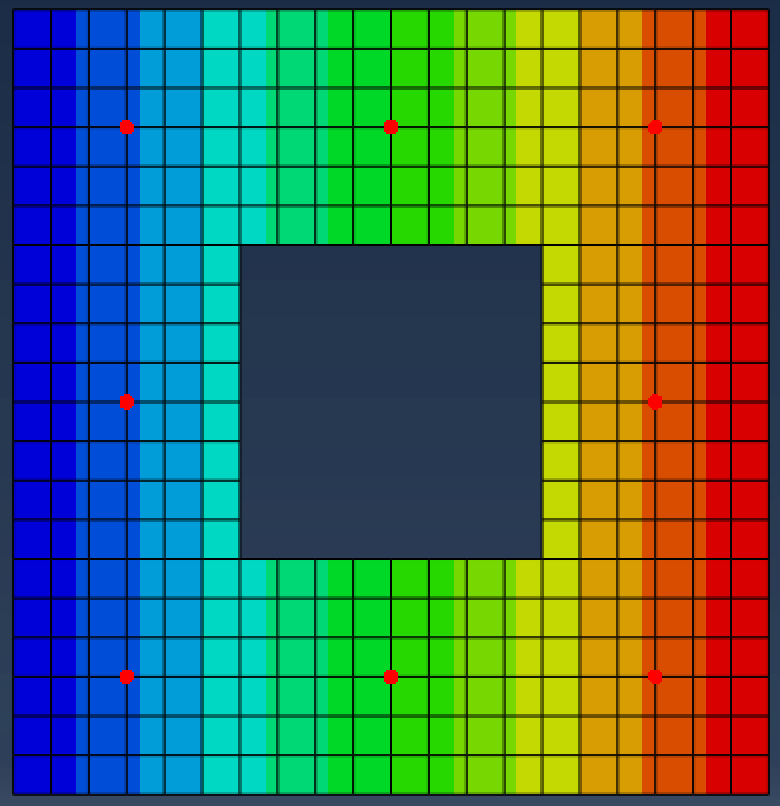
\includegraphics[width=0.4\textwidth]{Images/ab3/ab10.png} \qquad 
    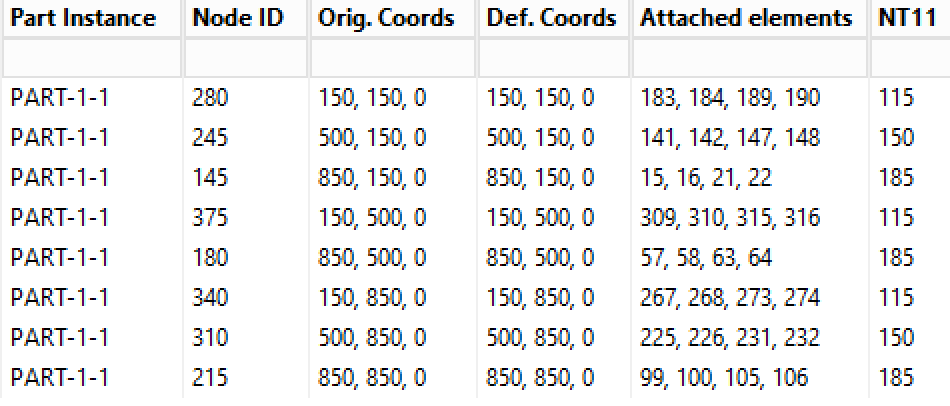
\includegraphics[width=0.5\textwidth]{Images/ab3/ab11.png}
    \caption{Nodal temperature of internal points.}
    \label{fig:abb1011}
\end{figure}

The numerical values are tabulated in the next section.

\newpage

\subsection{Comparison between MATLAB and Abaqus}
\label{sub:comparison4}%

Here we present the comparison of the results obtained from solving Problem 3 using MATLAB and Abaqus software. The comparison focuses on the temperature distribution at eight selected internal nodes, as depicted in Fig.~\ref{fig:2pr3f2}.

\begin{table}[H]
    %\caption*{\textbf{Title of Table (optional)}}
    \centering 
    \begin{tabular}{ccccc}
    \hline
    \rowcolor{bluepoli!40} % comment this line to remove the color
    Internal Point label & Abaqus label & Abaqus value & MATLAB value & UoM \\
    \hline
    1 & NT11 N:280 & 115 & 115.08022 & °C \\
    2 & NT11 N:245 & 150 & 150.26437 & °C \\
    3 & NT11 N:145 & 185 & 185.25460 & °C \\
    4 & NT11 N:375 & 115 & 115.07475 & °C \\
    5 & NT11 N:180 & 185 & 185.68733 & °C \\
    6 & NT11 N:340 & 115 & 115.08022 & °C \\
    7 & NT11 N:310 & 150 & 150.26347 & °C \\
    8 & NT11 N:215 & 185 & 185.25460 & °C \\
    \hline
    \end{tabular}
    \\[10pt]
    \caption{Nodal temperature results of Problem 3.}
    \label{table:stedyRes2}
\end{table}

The results presented in Table~\ref{table:stedyRes} demonstrate that the temperature values obtained from Abaqus and MATLAB are remarkably similar.

In addiction, these results perfectly match the ones obtained with FORTRAN in~\cite{sbemKatsi}, and they can be compared with the exact solution $u(x,y)=100(1+x)$, showing a rapid convergence.



